% -*- coding:utf-8 -*-
\documentclass{standalone}
\usepackage[UTF8]{ctex}
\usepackage{tikz}
\usepackage{amsmath}
\usetikzlibrary{matrix,calc,shapes,backgrounds,patterns,positioning,decorations.pathreplacing}
\begin{document}
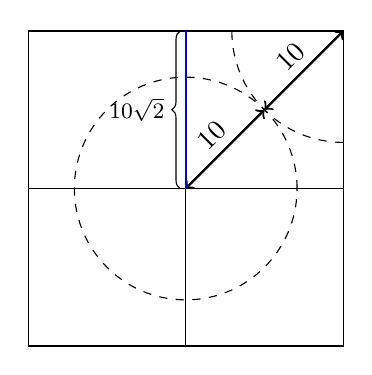
\begin{tikzpicture}
\draw[draw=black] (0,0) rectangle (2,2);
\draw[draw=black] (2,2) rectangle (4,4);
\draw[draw=black] (2,0) rectangle (4,2);
\draw[draw=black] (0,2) rectangle (2,4);
\draw[style=dashed] (2,2) circle (1.414213562373095);
\draw[style=dashed] (4,4-1.414213562373095) arc (-90:-180:1.414213562373095);
%\fill (2,2) circle (3pt);
\draw[thick, <->] (2,2) -- (3,3) node[pos=.5, sloped, above]{$10$};
\draw[thick, <->] (4,4) -- (3,3) node[pos=.5, sloped, above]{$10$};
\draw [decorate,decoration={brace,amplitude=3pt},xshift=-2pt,yshift=0pt]
(2,2) -- (2,4) node [black,midway,xshift=-0.55cm] 
{\footnotesize $10\sqrt{2}$};
\draw[thick, color=blue] (2,2) -- (2,4);
\end{tikzpicture}
\end{document}